% Este documento destina-se a servir como modelo para a produção de documentos
% de pesquisa do PPGINF/UFPR, como projetos, dissertações e teses. A classe de
% documento se chama "ppginf" (arquivo ppginf.cls) e define o formato básico do
% documento. O texto está organizado em capítulos que são colocados em
% subdiretórios separados. São definidos exemplos para a inclusão de figuras,
% códigos-fonte e a definição de tabelas.
%
% Produzido por Carlos Maziero (maziero@inf.ufpr.br) em Outubro de 2015.
% Adaptado de um modelo anterior construído pelo autor para o PPGIA/PUCPR.

% Opções da classe ppginf:
% - defesa: espaçamento 1,5, sem algumas páginas iniciais (default)
% - final:  espaçamento simples, completa
% - oneside: para impressão somente frente (default)
% - twoside: para impressão frente/verso
% - ... (demais opções aceitas pela classe "book")

% Opções default: defesa, oneside
\documentclass[defesa,oneside]{ppginf}
%\documentclass[final,twoside]{ppginf}

% configurações de diversos pacotes, inclusive o fonte principal do texto
% Pacotes usados neste documento e suas respectivas configurações

% ------------------------------------------------------------------------------

% Definição de fontes

% formato dos arquivos-fonte (utf8 no Linux e latin1 no Windows)
\usepackage[utf8]{inputenc}	% arquivos LaTeX em Unicode (UTF8)

% usar codificação T1 para ter caracteres acentuados corretos no PDF
\usepackage[T1]{fontenc}

% fonte usada no corpo do texto (descomente apenas uma)
\usepackage{newtxtext,newtxmath}	% Times (se não tiver, use mathptmx)
%\usepackage{lmodern}			% Computer Modern (fonte clássico LaTeX)
%\usepackage{kpfonts}			% Kepler/Palatino (idem, use mathpazo)
%\renewcommand{\familydefault}{\sfdefault} % Arial/Helvética (leia abaixo)

% A biblioteca central da UFPR recomenda usar Arial, seguindo a recomendação da
% ABNT. Essa é uma escolha ruim, pois fontes sans-serif são geralmente inade-
% quados para textos longos e impressos, sendo melhores para páginas Web.
% http://www.webdesignerdepot.com/2013/03/serif-vs-sans-the-final-battle/.

% fontes usadas em ambientes específicos
\usepackage[scaled=0.9]{helvet}		% Sans Serif
\usepackage{courier}			% Verbatim, Listings, etc

% ------------------------------------------------------------------------------

% inclusão de figuras em PDF, PNG, PS, EPS
\usepackage{graphicx}

% subfiguras (subfigure is deprecated, don't use it)
\usepackage[labelformat=simple]{subcaption}
\renewcommand\thesubfigure{(\alph{subfigure})}

% ------------------------------------------------------------------------------

% inclusão/formatação de código-fonte (programas)
\usepackage{listings}
\lstset{language=c}
\lstset{basicstyle=\ttfamily\footnotesize,commentstyle=\textit,stringstyle=\ttfamily}
\lstset{showspaces=false,showtabs=false,showstringspaces=false}
\lstset{numbers=left,stepnumber=1,numberstyle=\tiny}
\lstset{columns=flexible,mathescape=true}
\lstset{frame=single}
\lstset{inputencoding=utf8,extendedchars=true}
\lstset{literate={á}{{\'a}}1  {ã}{{\~a}}1 {à}{{\`a}}1 {â}{{\^a}}1
                 {Á}{{\'A}}1  {Ã}{{\~A}}1 {À}{{\`A}}1 {Â}{{\^A}}1
                 {é}{{\'e}}1  {ê}{{\^e}}1 {É}{{\'E}}1  {Ê}{{\^E}}1
                 {í}{{\'\i}}1 {Í}{{\'I}}1
                 {ó}{{\'o}}1  {õ}{{\~o}}1 {ô}{{\^o}}1
                 {Ó}{{\'O}}1  {Õ}{{\~O}}1 {Ô}{{\^O}}1
                 {ú}{{\'u}}1  {Ú}{{\'U}}1
                 {ç}{{\c{c}}}1 {Ç}{{\c{C}}}1 }

% ------------------------------------------------------------------------------

% formatação de algoritmos
\usepackage{algorithm,algorithmic}
\iflanguage{brazilian} {\floatname{algorithm}{Algoritmo}}{}
\renewcommand{\algorithmiccomment}[1]{~~~// #1}
%\algsetup{linenosize=\footnotesize,linenodelimiter=.}

% ------------------------------------------------------------------------------

% listas de símbolos e de abreviações (a fazer)
%\usepackage[titles]{tocloft}
%\newlistof[part]{symb}{los}{Lista de Símbolos}
%\newlistof[part]{abbrev}{loa}{Lista de Abreviações}
%\newcommand{\symb}[2]{%
%\refstepcounter{symb}
%\addcontentsline{los}{symb}{\protect #1 :#2}\par}

% ------------------------------------------------------------------------------

% formatação de bibliografia
\usepackage{natbib}		% bibliografia no estilo NatBib

% ------------------------------------------------------------------------------

% outros pacotes diversos
\usepackage{alltt,moreverb}	% mais comandos no modo verbatim
\usepackage{lipsum}		% gera texto aleatório (para os exemplos)
\usepackage{currfile}		% infos sobre o arquivo/diretório atual
\usepackage[final]{pdfpages}	% inclusão de páginas em PDF
\usepackage{longtable}		% tabelas multi-páginas (tab símbolos/acrônimos)

% ------------------------------------------------------------------------------



%=====================================================

\begin {document}

% Principais dados, usados para gerar as páginas iniciais.
% Campos não utilizados podem ser removidos ou comentados.

\title{Um modelo para dissertações e teses (escrevi um título mais longo para ver como se comporta a quebra de linhas e o espaçamento entre elas)}

% Estas devem ser definidas aqui para poder incorporar nos metadados do PDF
\pchave{palavra-chave 1, palavra-chave 2, palavra-chave 3}
\keyword{keyword 1, keyword 2, keyword 3}

\author{Carlos Alberto Maziero}
\advisor{Donald Knuth}
\coadvisor{Leslie Lamport}

\field{Ciência da Computação}	% default do PPGInf, não mudar

\date{2015}
\local{Curitiba PR}
\instit{UFPR}{Universidade Federal do Paraná}

%% Descrição do documento (obviamente, descomentar somente UMA!)

\descr{Tese apresentada como requisito parcial à obtenção do grau de Doutor em Informática no Programa de Pós-Graduação em Informática, setor de Ciências Exatas, da Universidade Federal do Paraná}

%\descr{Documento apresentado como requisito parcial para o exame de qualificação de Doutorado no Programa de Pós-Graduação em Informática, setor de Ciências Exatas, da Universidade Federal do Paraná}

%\descr{Dissertação apresentada como requisito parcial à obtenção do grau de Mestre em Informática no Programa de Pós-Graduação em Informática, setor de Ciências Exatas, da Universidade Federal do Paraná}

%\descr{Documento apresentado como requisito parcial para o exame de qualificação de Mestrado no Programa de Pós-Graduação em Informática, setor de Ciências Exatas, da Universidade Federal do Paraná}

%\descr{Trabalho apresentado como requisito parcial à conclusão do Curso de Bacharelado em XYZ, setor de Ciências Exatas, da Universidade Federal do Paraná}

%\descr{Trabalho apresentado como requisito parcial à conclusão da disciplina XYZ no Curso de Bacharelado em XYZ, setor de Ciências Exatas, da Universidade Federal do Paraná}

%=====================================================

% páginas iniciais (preâmbulo)
\frontmatter
\pagestyle{frontmatter}

% capa e folha de rosto
\titlepage

% páginas que só aparecem na versão final (seleção automática)
% - IMPORTANTE - IMPORTANTE - IMPORTANTE - IMPORTANTE -
%
% O conteúdo exato da ficha catalográfica é preparada pela Biblioteca Central
% da UFPR, a pedido da secretaria do PPGINF. Não "invente" um conteúdo para ela,
% se informe a respeito com nossa secretária.

\begin{ficha}	% só gera conteúdo se for na versão final

% "Ficha" provisória (comentar quando tiver a ficha oficial)
\begin{center}
\textbf{Ficha Catalográfica}

~

\emph{Esta folha deve ser substituída pela ficha catalográfica fornecida pela Biblioteca Central da UFPR, a pedido da secretaria do PPGInf/UFPR (vide arquivo \texttt{ficha.tex}).}
\end{center}

% para a inclusão da ficha catalográfica final em formato PDF
%\includepdf[\thispagestyle{empty},noautoscale]{ficha.pdf}

\end{ficha}

%=====================================================
	% ficha catalográfica
% A ficha de aprovação será fornecida pela secretaria do programa,
% após a defesa e cumprimento dos demais trâmites legais.

\begin{aprovacao}	% só gera conteúdo se for na versão final

% "Texto" provisório (remover quando tiver a aprovacao oficial)
\begin{center}
\textbf{Termo de aprovação}

~

\emph{Esta folha deve ser substituída pela ata de defesa ou termo de aprovação devidamente assinado, que será fornecido pela secretaria do programa após a defesa ter sido concluída e aprovada (vide arquivo \texttt{aprovacao.tex}).}
\end{center}

% para a inclusão da aprovacao final em formato PDF:
%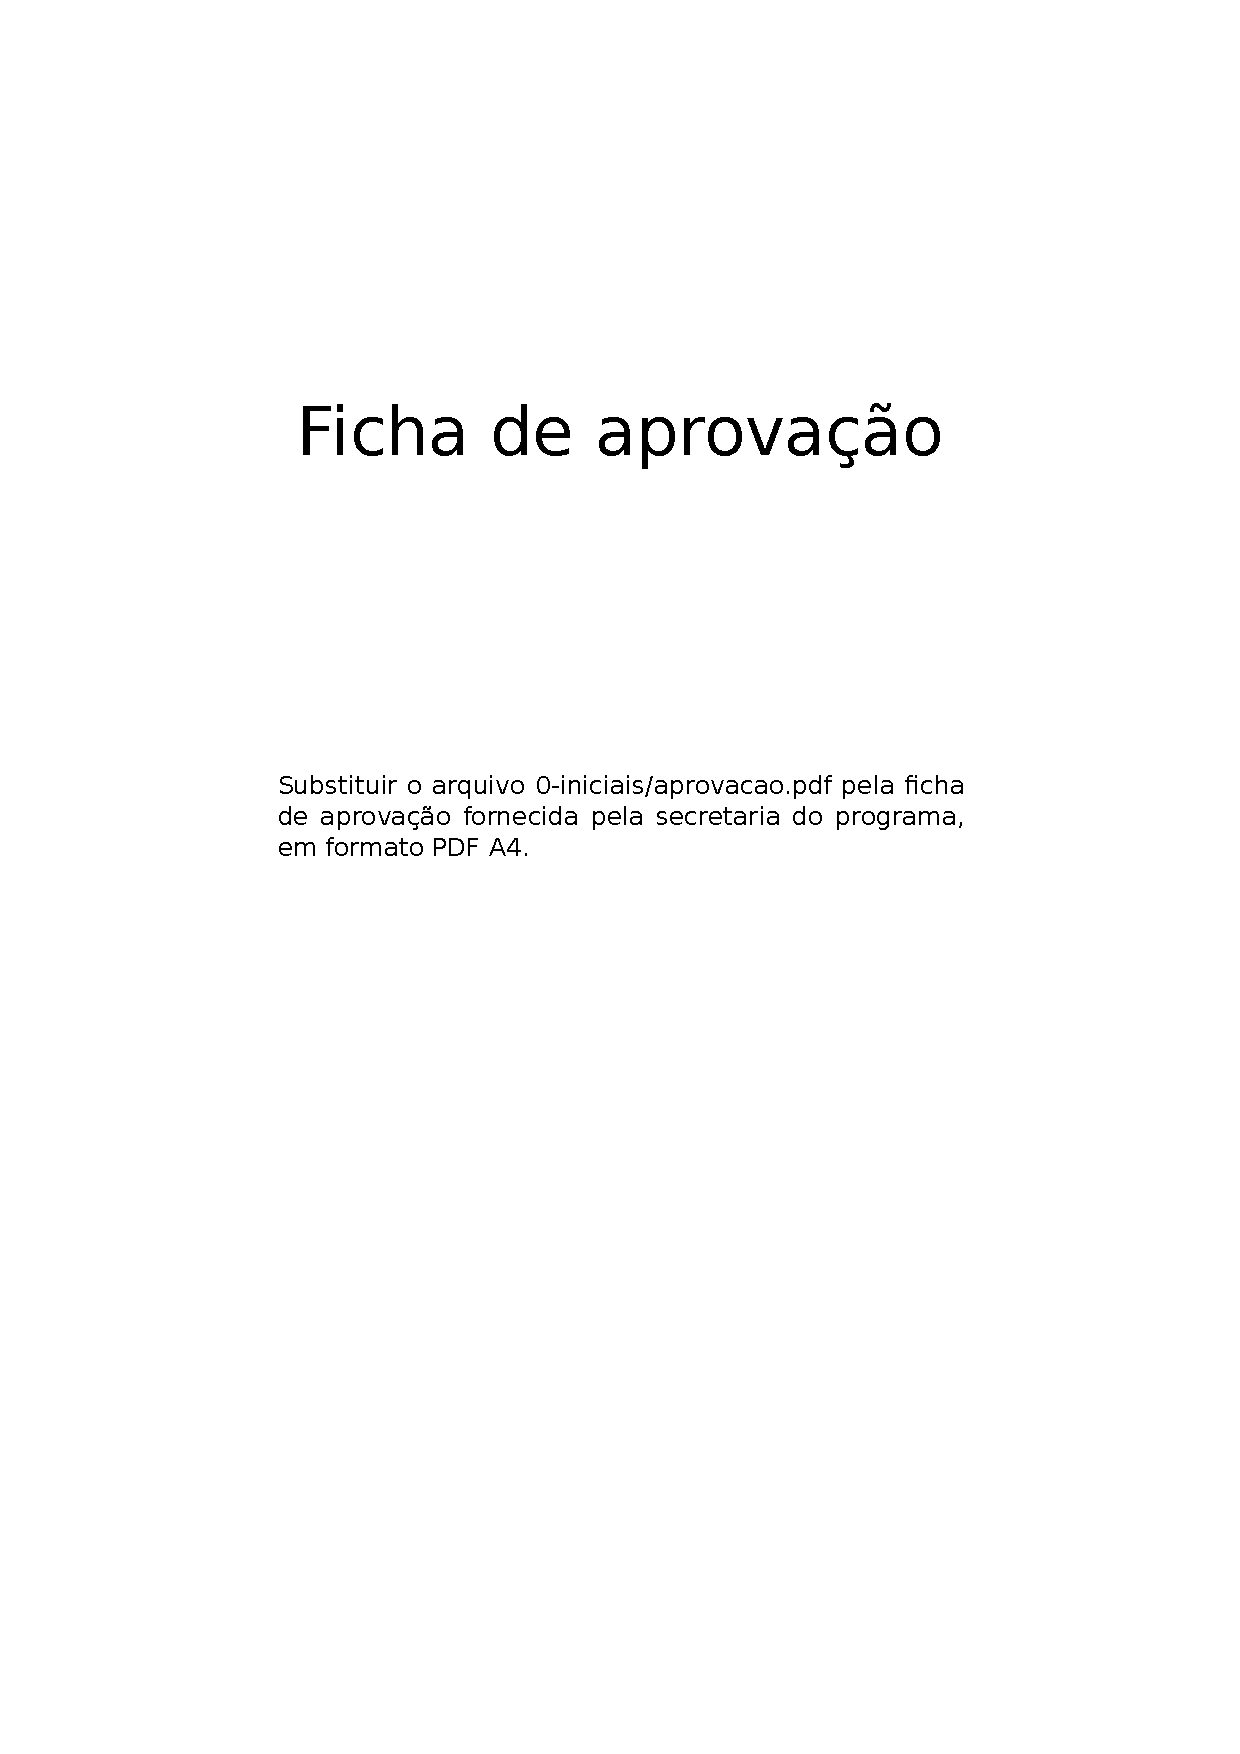
\includepdf[\thispagestyle{empty},noautoscale]{aprovacao.pdf}

\end{aprovacao}

%=====================================================
	% folha de aprovação
\begin{dedica}  % só gera conteúdo se for na versão final

A alguém...

\end{dedica}

	% dedicatória
\begin{agradece}	% só gera conteúdo se for na versão final

Inserir os agradecimentos. Os agradecimentos devem ocupar no máximo uma página, devem ser justificados na largura da página e com um afastamento de parágrafo na primeira linha de 1,27 cm. O espaçamento entre linhas deve ser de 1,5 linhas. Não deve haver espaçamento adicional entre parágrafos.

\lipsum[2-5]	% gera um texto aleatório

\end{agradece}

	% agradecimentos

% resumo e abstract
\begin{resumo}

O resumo deve conter no máximo 500 palavras, devendo ser justificado na largura da página e escrito em um único parágrafo\footnote{E também não deve ter notas de rodapé; em outras palavras, não siga este exemplo... ;-)} com um afastamento de 1,27 cm na primeira linha. O espaçamento entre linhas deve ser de 1,5 linhas. O resumo deve ser informativo, ou seja, é a condensação do conteúdo e expõe finalidades, metodologia, resultados e conclusões.

\lipsum[11-14]	% texto aleatório

\end{resumo}


\begin{otherlanguage}{english}

\begin{abstract}

% em inglês, o primeiro parágrafo não deve ser indentado
\noindent
The abstract should be the English translation of the ``resumo'', no more, no less.

\end{abstract}

\end{otherlanguage}



% sumário e demais listas (figuras, tabelas, abreviações/siglas, símbolos)
\tableofcontents
\listoffigures
\listoftables
%=====================================================

% lista de acrônimos (siglas e abreviações)

\begin{listaacron}

\begin{longtable}{ll}
DINF & Departamento de Informática\\
PPGINF & Programa de Pós-Graduação em Informática\\
UFPR & Universidade Federal do Paraná\\
\end{longtable}

\end{listaacron}

%=====================================================
	% ainda deve ser preenchida à mão
%=====================================================

% lista de símbolos

\begin{listasimb}

\begin{tabular}{ll}
$\alpha$ & alfa, primeira letra do alfabeto grego\\
$\beta$ & beta, segunda letra do alfabeto grego\\
$\gamma$ & gama, terceira letra do alfabeto grego\\
$\omega$ & ômega, última letra do alfabeto grego\\
$\pi$ & pi \\
$\tau$ & Tempo de resposta do sistema\\
$\theta$ & Ângulo de incidência do raio luminoso\\
\end{tabular}

\end{listasimb}

%=====================================================
	% idem

%=====================================================

% corpo do documento
\mainmatter
\pagestyle{mainmatter}

% inclusao de cada capítulo, alterar a gosto (do professor de Metodologia)
\chapter{Introdução}

%=====================================================

% A introdução geral do documento pode ser apresentada através das seguintes seções: Desafio, Motivação, Proposta, Contribuição e Organização do documento (especificando o que será tratado em cada um dos capítulos). O Capítulo 1 não contém subseções\footnote{Ver o Capítulo \ref{cap-exemplos} para comentários e exemplos de subseções.}.

Este modelo foi proposto com o intuito de padronizar e simplificar as monografias, dissertações e teses produzidas no Departamento de Informática da UFPR. Ele foi vagamente inspirado nas normas da ABNT (conforme indicado em \cite{bibufpr15}), mas não as segue \emph{ipsis litteris}. Várias alterações foram feitas com o objetivo de melhorar sua estética e tornar o texto mais legível para trabalhos na área de informática. A versão atualizada deste modelo está disponível em \cite{maziero15}.

Este modelo está baseado em uma classe especifica \verb#ppginf.cls#, que aceita várias opções de compilação. A versão do documento pode ser:

\begin{itemize}

\item \verb#defesa#: é gerado um documento em espaço 1,5, frente simples e sem as páginas iniciais adicionais; é uma versão adequada para receber as anotações dos membros da banca de defesa.

\item \verb#final#: é gerado um documento em espaço simples, frente/verso, com páginas iniciais (capa, ficha catalográfica, folha de aprovação, agradecimentos, etc). É uma versão bem mais compacta, mais ecológica e ideal para a impressão definitiva.

\end{itemize}

Para obter os melhores resultados, compile este modelo usando a seguinte sequência de passos:

\begin{quote}
\begin{footnotesize}
\begin{verbatim}
pdflatex  main          // compilação inicial
bibtex main             // processa referências bibliográficas
pdflatex  main          // compilação final
\end{verbatim}
\end{footnotesize}
\end{quote}

ou

\begin{quote}
\begin{footnotesize}
\begin{verbatim}
make                    // faz tudo...
\end{verbatim}
\end{footnotesize}
\end{quote}

Os principais itens considerados na formatação deste documento foram:

\begin{itemize}

\item Papel em formato A4, com margens de 20 mm à direita e embaixo, 30 mm nos demais lados. Não devem ser usados cabeçalhos ou rodapés além dos que estão aqui propostos.

\item O texto principal do documento escrito em 12 pontos. O fonte principal do texto pode ser selecionado no arquivo \verb#packages.tex#.

\item Código-fonte, listagens e textos similares são formatados em fonte Courier 12 ou 10 pontos.

\item O espaçamento padrão entre linhas é 1,5 linhas (1 linha na versão final). Não inserir espaços adicionais entre parágrafos normais. Figuras, tabelas, listagens e listas de itens devem ter um espaço adicional antes e após os mesmos.

\item As páginas iniciais não são numeradas.

\item O corpo do texto é numerado com algarismos arábicos (1, 2, 3, ...) a partir da introdução, ate o final do documento. Os números de página devem estar situados no alto à direita (páginas direitas) ou à esquerda (páginas esquerdas).

\item Expressões em inglês, grego, latim ou outras línguas devem ser enfatizadas em itálico, como \emph{sui generis} ou \emph{scheduling} (use o comando \verb#\emph{...}#).

\item Para reforçar algo, deve-se usar somente \textbf{negrito}. \underline{Sublinhado} ou MAIÚSCULAS não devem ser usados como forma de ênfase!

\item As notas de rodapé também têm um modelo\footnote{As notas de rodapé dever ser escritas em tamanho 10 pt, numeradas em arábico.}. Notas de rodapé servem para fazer algum comentário paralelo; não as use para colocar URLs, referências bibliográficas ou significado de siglas.

\end{itemize}

Felizmente o \LaTeX\ resolve a maior parte dessas questões!

%=====================================================
		% introdução
\chapter{Alguns exemplos}
\label{cap:exemplos}

% figuras estão no subdiretório "figuras/" dentro deste capítulo
\graphicspath{\currfiledir/figuras/}

%=====================================================

\section{Guias de \LaTeX}

Este modelo contém exemplos para os padrões de inserção de figuras, tabelas, listas de itens, bibliografia, etc. Em caso de dúvidas ou discordância, Pode-se entrar em contato com a direção ou secretaria do programa. Obviamente, críticas (construtivas) e sugestões são muito bem-vindas.

Para aprender a usar \LaTeX, um bom guia introdutório disponível na Internet é \cite{oetiker07}, que também tem uma versão em português. Para tópicos mais avançados consulte \cite{goossens93}.

%=====================================================

\section{Estrutura do texto}

Para melhorar a legibilidade do texto, deve ser extremamente evitado o uso de subdivisões mais profundas que a subseção (por exemplo, subsubseções). Se elas forem absolutamente necessarias, não devem ser numeradas. Deve-se analisar a possibilidade de uso de uma lista de itens em seu lugar. O número de níveis de texto do documento não deve exceder três: capítulo, seção e subseção. O uso de mais que três níveis dificulta a leitura e prejudica muito a estética do texto.

%=====================================================

\section{Estilo de redação}

Ao elaborar o texto da dissertação ou da tese, o mais indicado é o uso do verbo na forma impessoal. Exemplos:

\begin{itemize}
\item ... utilizaram-se os seguintes dados ...
\item ... elaborou-se de forma precisa ...
\item ... trata-se os algoritmos ...
\item ... foram obtidos resultados significativos ...
\end{itemize}

Além disso, deve-se a todo custo evitar a ``linguagem de revista'', com expressões como ``sensacional'', ``impressionante'', ``monstruoso'', etc (por exemplo: ``Os resultados obtidos são sensacionais, sobretudo considerando a monstruosa margem de erro.'').

%=====================================================

\section{Exemplo de figura}

A forma sugerida para incluir figuras em um documento \LaTeX\ é importá-las usando o pacote \texttt{graphicx}. Como formatos gráficos sugere-se:

\begin{itemize}

\item Formatos \emph{raster}, como PNG (\emph{Portable Network Graphics}) ou JPG (\emph{Joint Photographic Experts Group}) para fotografias; procure usar uma resolução de ao menos 150 dpi (\emph{dots per inch}).

\item Formatos vetoriais, como PDF (\emph{Portable Document Format}) ou EPS (\emph{Extended PostScript}) para diagramas e gráficos\footnote{NUNCA use JPG ou GIF para desenhos vetoriais, pois o resultado final geralmente fica borrado.}.

\end{itemize}

A maior parte das ferramentas permite exportar figuras nesses formatos (a figura do exemplo foi produzida com o \emph{Inkscape}, um programa livre multiplataforma). A figura \ref{fig:comun-intra-inter} mostra um exemplo de inclusão de figura em PDF.

% exemplo de inserção de figura
\begin{figure}[!htb]
\centering
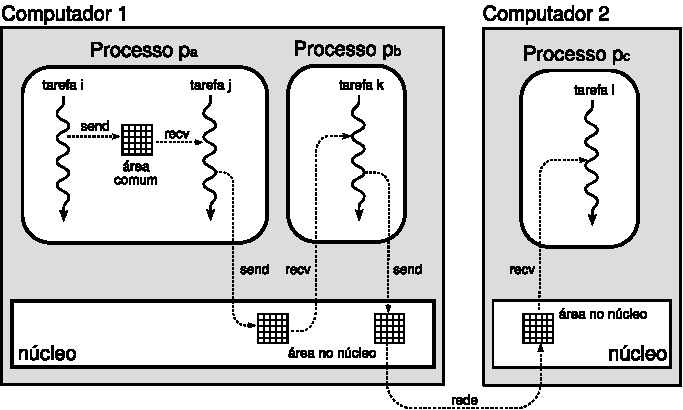
\includegraphics[width=12cm]{exemplo-figura.pdf}
\caption{Comunicação inter-processos.}
\label{fig:comun-intra-inter}
\end{figure}

Para mais informações consulte \cite{goossens93}.

%=====================================================

\section{Exemplo de tabela}

Tabelas são elementos importantes de um documento. No \LaTeX\ as tabelas podem ser objetos flutuantes (definidas no ambiente \texttt{table} e referenciadas por números usando \texttt{label} e \texttt{ref}) ou objetos fixos simples, criados pelo ambiente \texttt{tabular}. A tabela \ref{tab:modelos} é um exemplo de tabela flutuante, cuja posição no texto pode variar em função das quebras de página.

\begin{table}[!htp]
\centering
\caption{Os 16 modelos centrais do UCON$_{\mathrm{ABC}}$}
\label{tab:modelos}
\begin{tabular}{|c|cccc|}
\cline{2-5}
\multicolumn{1}{c|}{}& 0 (imutável) & 1 (\emph{pre-update}) & 2 (\emph{on-update}) & 3 (\emph{pos-update}) \\
\hline
\texttt{preA} & \textbullet & \textbullet & -- & \textbullet \\
\hline
\texttt{onA} & \textbullet & \textbullet & \textbullet & \textbullet \\
\hline
\texttt{preB} & \textbullet & \textbullet & -- & \textbullet \\
\hline
\texttt{onB} & \textbullet & \textbullet & \textbullet & \textbullet \\
\hline
\texttt{preC} & \textbullet & -- & -- & -- \\
\hline
\texttt{onC} & \textbullet & -- & -- & -- \\
\hline
\end{tabular}
\end{table}

%=====================================================

\section{Exemplo de equação}

Equações destacadas devem ser numeradas como mostra a equação \ref{eq:relatividade}:

\begin{equation}
E = m \times c^2
\label{eq:relatividade}
\end{equation}

%=====================================================

\section{Exemplos de código-fonte}

Códigos-fonte podem ser produzidos de forma simples através do ambiente \texttt{verbatim}, como mostra este exemplo:

\begin{footnotesize}
\begin{verbatim}
#include <stdio.h>

int main (int argc, char *argv[])
{
   int i ;                           // uma variavel local

   for (i=0; i< 100; i++)            // um laço for
      printf ("i vale %d\n", i) ;    // uma saída na tela
}
\end{verbatim}
\end{footnotesize}

No entanto, é preferível usar pacotes especializados para a edição ou inclusão de códigos-fonte, como o pacote \texttt{listings}. Eis um exemplo de código-fonte escrito com esse pacote:

% exemplo de código-fonte definido no próprio texto

\begin{lstlisting}
#include <stdio.h>

int main (int argc, char *argv[])
{
   int i ;                           // uma variável local

   for (i=0; i< 100; i++)            // um laço for
      printf ("i vale %d\n", i) ;    // uma saída na tela
}
\end{lstlisting}

Esse pacote também permite incluir códigos-fonte de arquivos externos. Eis um exemplo:

% exemplo de código-fonte incluso

\lstinputlisting{2-fundam/exemplo.c}

%=====================================================

\section{Exemplo de algoritmo}

Os pacotes \texttt{algorithm} e \texttt{algorithmic} permitem formatar algoritmos facilmente. Eis um exemplo:

\begin{algorithm}[H]
\caption{Ações de $s_i$ ao encerrar um ciclo:}
\label{alg:on-period-ending}
\begin{small}
\begin{algorithmic}[1]
\FORALL{$x \in \mathcal{K}_i$}
  \STATE{$\mathit{banned}_i(x) \gets$ FALSE}
  \STATE{$mi_i(x) \gets 0$}
  \STATE{$mm_i(x) \gets 0$}
  \STATE{$\mathit{age}_i(x) \gets \mathit{age}_i(x) + 1$}
  \IF{$\mathit{age}_i(x) = \mathit{age}_\mathit{max}$}
     \STATE{$\mathcal{K}_i \gets \mathcal{K}_i - \{x\}$}
     \COMMENT{``esquece'' do servidor $x$}
     \STATE{remove as informações locais sobre $x$}
     \STATE{envia $\mathit{notify}(x,\mathit{undef})$ ao grupo de confiança $\mathcal{T}_i$}
  \ENDIF
\ENDFOR
\end{algorithmic}
\end{small}
\end{algorithm}
 
%=====================================================

\section{Conclusão}

Todo capítulo (com exceção da introdução e da conclusão) deve encerrar com uma pequena conclusão local, resumindo os tópicos apresentados no capítulo e preparando o leitor para o próximo capítulo (exceto se esse for a conclusão geral). Caso o capítulo tenha apresentado resultados obtidos pelo próprio autor, estes devem ser sucintamente relembrados aqui.

%=====================================================
	% fundamentação teórica
\include{3-revbib/revbib}	% revisão bibliográfica (estado da arte)
\include{4-proposta/proposta}	% proposta
\include{5-valida/valida}	% experimentação e validação
\include{6-conclusao/conclusao}	% conclusão

%=====================================================

% Estilos de bibliografia recomendados (só descomentar um estilo!)
\bibliographystyle{apalike}	% [Maziero, 2007], [Maziero et al., 2006]
%\bibliographystyle{plain}	% [1], [1, 2]

% base de bibliografia (BibTeX)
\bibliography{refs}
%\bibliography{ref1, ref2, ref3} % se tiver mais de um arquivo BibTeX

%=====================================================

% apêndices
\appendix
\chapter{Exemplo de anexo}

%=====================================================

Os apêndices são uma extensão do texto, destacados deste para evitar descontinuidade na sequência lógica ou alongamento excessivo de determinado assunto ou tópico secundário dentro dos capítulos da dissertação ou da tese. São contribuições que servem para esclarecer, complementar, provar ou confirmar as ideias apresentadas no texto dos capítulos e que são importantes para a compreensão dos mesmos.

Todos os apêndices devem vir após as referências bibliográficas e devem ser enumerados por letras maiúsculas (A, B, C, ...).

%=====================================================

\section{Uma Seção}

\lipsum[20-23]

%=====================================================

\subsection{Uma sub-Seção}

\lipsum[30-33]

%=====================================================


\end{document}

%=====================================================
